\documentclass[notitlepage]{report}
\usepackage[utf8]{inputenc} % Prendre en compte les caractères accentués
%\usepackage[francais]{babel} % Prendre en compte les particularités de la typographie française.
\usepackage{geometry}         % marges
\usepackage{graphicx}         % images
\usepackage{setspace}
%\usepackage[french]{varioref}
\usepackage{titlesec}
\usepackage{parskip}
\usepackage{url}
\usepackage{verbatim}
\usepackage{caption}
\usepackage{enumitem}
\usepackage{ragged2e}
\usepackage{xcolor}
\usepackage{textcomp}
\usepackage{listings}
\usepackage{pgfgantt}
\usepackage{lscape}
\usepackage{pdfpages}
\usepackage{supertabular} % tableaux qui tiennent sur plusieurs pages
\usepackage{multirow} % plusieur ligne dans une ligne de tableau
\usepackage{pdflscape} % Automatic rotation of the landscape page
\usepackage{colortbl} %Couleur de fond tableau
\usepackage{lipsum,etoolbox} %Pour que l'abstract se mette dans la ToC

\titlespacing{\chapter}{0pt}{*-5}{*5}
\titlespacing{\section}{0pt}{*2}{*2}
\titleformat{\chapter}[hang]{\bf\huge}{\thechapter}{2pc}{}
%\titleformat{\chapter}[hang]{\bf\huge}{\thechapter}{14pt}{\LARGE}
\renewcommand{\baselinestretch}{1.2}
\setlength{\parskip}{1.5ex plus .4ex minus .4ex}
\setlength{\parindent}{15pt} 
\setlength{\topmargin}{-35pt}
\setlength{\textheight}{600pt}

\makeatletter
% subsubsubsection
\newcounter{subsubsubsection}[subsubsection] 
\renewcommand\thesubsubsubsection{\@roman\c@subsubsubsection}
\newcommand\subsubsubsection{\@startsection{subsubsubsection}{4}{\z@}%
                                     {-3.25ex\@plus -1ex \@minus -.2ex}%
                                     {1.5ex \@plus .2ex}%
                                     {\normalfont\small\bfseries}}
\newcommand*\l@subsubsubsection{\@dottedtocline{3}{5.2em}{1em}}
\newcommand*{\subsubsubsectionmark}[1]{}
\setcounter{secnumdepth}{2}
\makeatother

\title{\textbf{User manual}\\sig\_ros package}
\author{}
\date{\today}

\begin{document}
\maketitle
%\sloppy % Justification moins stricte : des mots ne dépasseront pas des paragraphes


%%\chapter*{Remerciements}
%\setlength{\parskip}{2.5ex plus .4ex minus .4ex}
\setcounter{page}{2} 
%Je tiens à remercier certaines personnes sans lesquelles ce stage n'aurait pas eu lieu.\\
%Hélène Raynal, responsable du projet RECORD\footnote{Rénovation et CooRDination de la modélisation de cultures pour la gestion des agro écosystèmes}, Gauthier Quesnel du projet VLE\footnote{Virtual Laboratory Environment}, appartenants au département MIA\footnote{Mathématiques et Informatique Appliquées}.\\
%Laurence Puillet et Olivier Martin, du projet Archimod, département PHASE\footnote{PHysiologie Animale et Systèmes d’Élevage} qui ont exprimé les besoins et sont les principaux futurs utilisateurs ainsi que Régis Sabbadin, Directeur de l'Unité MIAT\footnote{Mathématiques et Informatique Appliquées de Toulouse}, lieu de déroulement du stage.\\
%
%Merci également à mon maître de stage Patrick Chabrier pour ses explications et conseils tout au long du stage ainsi que les stagiaires présents dans l'entreprise qui m'ont aidé et rendu le temps passé dans l'entreprise très agréable.\\
%
%Je souhaite également remercier toutes les personnes au sein de l'école Polytech'Nice qui ont rendu ce stage possible.
\renewcommand{\abstractname}{Gratitude}
\vspace*{\fill}
\begin{abstract}
%\addcontentsline{toc}{chapter}{Gratitude}
I wish to thank the National Institute of Informatics who gave me the opportunity to do my six-month internship in one of its laboratory. With this internship, I finalize my master's degree in computer science engineering.\\

I also want to thank my supervisor, Inamura \textsc{Tetsunari} associate professor, for his time invested, his interest in my study and for all the knowledge he helped me deepen.\\

I thank the National Institute of Informatics administration staff who helped me get over all administrative steps and my interrogations. Also a thank you to Polytech'Nice Sophia who make this internship possible.\\

Finally I would like to say many thanks to all the people who made my study and internship possible, and encourage me during my all study - friends, familly and the all people I met who gave me good moment.
\end{abstract}
\vspace*{\fill}
\renewcommand{\abstractname}{Abstract}

 
\tableofcontents % Table des matières
\setcounter{page}{2}
\chapter{Generalities}
\section{Goal}
This package aim to provide a tool for using SIGVerse\cite{SIGVerseWiki} though ROS without knowledge of SIGVerse or limited knowledge.\\
Using sig\_ros package will allow you to send topics and call services directly to SIGVerse.

\section{For who?}
This package is intended for ROS users or SIGVerse users who want to use SIGVerse in a different way.\\
For using this package you previously need basic knowledge of ROS, that means at least the beginner level of the ROS tutorials page\cite{ROSWiki}, running a node, publishing and subscribing to a topic, calling a service...is the minimum requiered.

\section{Install}
First of all, you have to install SIGServer\cite{SIGServerWiki} and SIGViewer\cite{SIGViewerWiki} like explained in the SIGVerse wiki page\cite{SIGVerseWiki}.

\noindent\textbf{Create a catkin workspace:} 
\begin{lstlisting}[language=bash]
mkdir -p ~/catkin_ws/src
\end{lstlisting}
\textbf{Initialize the workspace:} 
\begin{lstlisting}[language=bash]
cd ~/catkin_ws/src
catkin_init_workspace
cd ..
catkin_make
source devel/setup.bash
\end{lstlisting}
\textbf{Clone the git repository:}
\begin{lstlisting}[language=bash]
git clone https://github.com/GG31/sig_ros.git
\end{lstlisting}
\textbf{Change the name of sig\_ros folder you've just cloned by src, so you have the tree:}
\begin{lstlisting}[language=bash]
|-- catkin_ws
    |-- src
        |-- sig_ros
        |-- user
    |-- devel
    |-- build
\end{lstlisting}
\textbf{Change the absolute links on \url{catkin_ws/src/user/xml/CleanUpDemo2014.xml} there is 5, on \url{catkin_ws/src/sig_ros/src/ros_controller.cpp} there is one and on \url{catkin_ws/src/sig_ros/CMakeLists.txt}}\\
\textbf{Create libsig\_ros:} 
\begin{lstlisting}[language=bash]
mkdir ~/catkin_ws/devel/lib/libsig_ros
\end{lstlisting}

\chapter{Usage}
The repository \url{https://github.com/GG31/sig_ros.git} contains two package sig\_ros and user. sig\_ros is the package who make the interface between SIGVerse and ROS and user is an example of package who contains severals nodes. These nodes send messages and call services who reproduce the clean up task demo.\\
On the directory \url{~/catkin_ws/src/user/xml} there are the all xml file needed by the clean up task.\\

Go to the directory \url{~/catkin_ws/src/user/xml} and run the ros\_controller node of the sig\_ros package with:
\begin{lstlisting}[language=bash]
cd ~/catkin_ws/src/user/xml
rosrun sig_ros ros_controller CleanUpDemo2014Robot.xml
\end{lstlisting}
The SIGServer is launched automatically and you and see the number of the port.\\
Find the IP address with ifconfig.\\
Then open the SIGViewer and write the IP adress and the port. Click on ``Connect''. It is the step 1 in the figure~\ref{fig:usage}.\\
After that, you can see the world defined by the xml files, if the camera is not well positionned, do not hesitate to move it with the mouse and the keys Ctrl, Alt and Maj.\\

Start the simulation, the all topics and services are created at the same time. This is the step 2 in figure~\ref{fig:usage}. After that, you will be able to publish, subscribe and call a service.\\
You can see figure~\ref{fig:usage} a sum up of the three steps. During the third step you can create all the node you want and communicate with SIGVerse.\\
For example, in the package user, there are severals node which can be started, ``RobotCommand'', ``ModeratorCommand'',...\\
Start the ``RobotCommand'' node.
\begin{lstlisting}[language=bash]
rosrun user RobotCommand
\end{lstlisting}
The robot will begin to move.\\
If you start the service ``Referee'' and the ``ModeratorCommand'' node, the score will be counted.

\noindent\begin{minipage}{\linewidth}% to keep image and caption on one page
\makebox[\linewidth]{%        to center the image
  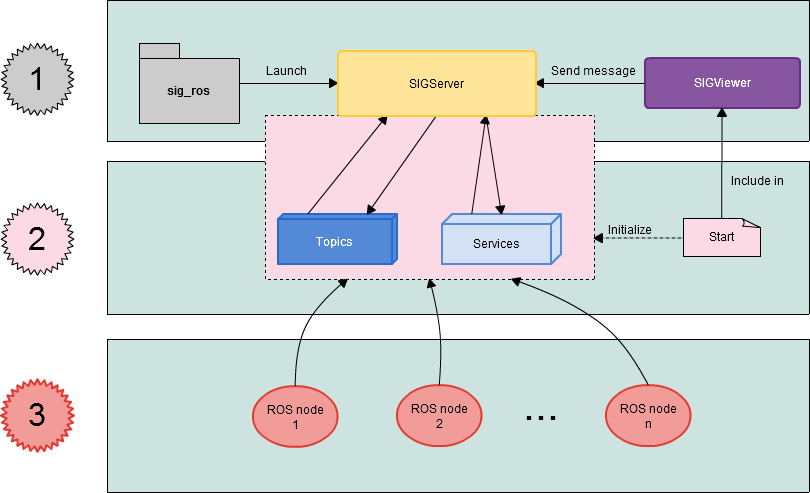
\includegraphics [width=140mm]{images/usage.png}}
\captionof{figure}{Usage of the package}\label{fig:usage}  
\end{minipage}

\chapter{Topics}
For all the topics, if there is a parameters called ``name'', that means it refers to an entity. For example, if we have the topic robot\_000\_setPosition if the parameter ``name'' is filled by ``trashbox\_0'', the topic will set the position to the trashbox, but if the parameter ``name'' is an empty string, then it will be the ``robot\_000''. For the services, the parameter ``name'' works as well.\\

\begin{supertabular}{|p{2.9cm}|p{4.5cm}|p{7cm}|}
	\hline
    Topic name & Message & Description \\
  	\hline
  	\_onRecvMsg &
  		\textbf{sender} : string\newline 
  		\textbf{content} : string
  		\medskip & The ``Controller'' send the message received by the SIGViewer.\\
  	\hline
  	\medskip
  	\_onCollisionMsg &
  		\medskip
  		\textbf{name} : string \newline
  		\textbf{part} : string & The name of the agent which one is in collision with are sent to this topic. If there is severals collision at the same time, severals messages are sent.\\
  	\hline
  	\_setWheel & 
  		\textbf{wheelRadius} : double \newline
  		\textbf{wheelDistance} : double & Publish the radius and the distance in a message and they will be applied to the robot.\\
  	\hline
  	\_setWheelVelocity & 
  		\textbf{leftWheel} : double \newline
  		\textbf{rightWheel} : double
  		& Publish the velocity for the left and the right wheel and it will be applied.\\
  	\hline
  	\_setJointVelocity & 
  		\textbf{jointName} : string\newline
  		\textbf{angularVelocity} : double \newline
  		\textbf{max} : double
  		& jointName, angular velocity, max ???\\
  	\hline
  	\_releaseObj & \textbf{arm} : string & Publish the part which you want to release an object and it will be done.\\
  	\hline
  	\_setAxisAndAngle & 
  		\textbf{name} : string \newline
  		\textbf{axisX} : double \newline
  		\textbf{axisY} : double \newline
  		\textbf{axisZ} : double \newline
  		\textbf{angle} : double
  		& Set the axis defined by ``axisX'', ``axisY'' and ``axisZ'' and set the angle ``angle'' to the entity called ``name'', if no name is provided, the main entity of the topic will be set.\\
  	\hline
  	\_setPosition & 
  		\textbf{name} : string \newline
  		\textbf{posX} : double \newline
  		\textbf{posY} : double \newline
  		\textbf{posZ} : double
  		& Set the position ``posX'', ``posY'' and ``posZ'' to the entity called ``name'', if no name is provided, the main entity of the topic will be set.\\
  	\hline
  	\_setAccel & 
  		\textbf{name} : string \newline
  		\textbf{x} : double \newline
  		\textbf{y} : double \newline
  		\textbf{z} : double
  		& Set the acceleration to the entity\\
  	\hline
  	\_setAngularVelocity & 
  		\textbf{name} : string \newline
  		\textbf{x} : double \newline
  		\textbf{y} : double \newline
  		\textbf{z} : double
  		& Set angular velocity to the entity name (only in Dynamics ON)\\
  	\hline
  	\_setTorque & 
  		\textbf{name} : string \newline
  		\textbf{x} : double \newline
  		\textbf{y} : double \newline
  		\textbf{z} : double
  		& Set the torque.\\
  	\hline
  	\_setVelocity & 
  		\textbf{name} : string \newline
  		\textbf{x} : double \newline
  		\textbf{y} : double \newline
  		\textbf{z} : double
  		& Set Velocity to the entity.\\
  	\hline
  	\_setCollisionEnable & 
  		\textbf{name} : string \newline
  		\textbf{flag} : boolean
  		& Set if the collision is enable, true, false otherwise.\\
  	\hline
  	\_setGravityMode & 
  		\textbf{name} : string \newline
  		\textbf{boolean} : boolean
  		& Set the gravity mode, true if enable, false otherwise.\\
  	\hline
  	\_setJointAngle & 
  		\textbf{name} : string \newline
  		\textbf{jointName} : string \newline
  		\textbf{angle} : double
  		& Set the angle of the joint (only in Dynamics OFF).\\
  	\hline
  	\_setJointQuaternion & 
  		\textbf{name} : string \newline
  		\textbf{jointName} : string \newline
  		\textbf{qW} : double \newline
  		\textbf{qX} : double \newline
  		\textbf{qY} : double \newline
  		\textbf{qZ} : double \newline
  		\textbf{offset} : boolean 
  		& Set the quaternion of joint (only in Dynamics OFF).\\
  	\hline
  	\_setMass & 
  		\textbf{name} : string \newline
  		\textbf{mass} : double
  		& Set the mass of the entity .\\
  	\hline
  	\_addForce & 
  		\textbf{name} : string \newline
  		\textbf{x} : double \newline
  		\textbf{y} : double \newline
  		\textbf{z} : double
  		& Add force to a body using absolute coordinates (only in Dynamics ON).\\
  	\hline
  	\_setForce & 
  		\textbf{name} : string \newline
  		\textbf{x} : double \newline
  		\textbf{y} : double \newline
  		\textbf{z} : double
  		& Set the force applied to the entity (only in Dynamics ON).\\
  	\hline
  	\_addForceAtPos & 
  		\textbf{name} : string \newline
  		\textbf{x} : double \newline
  		\textbf{y} : double \newline
  		\textbf{z} : double \newline
  		\textbf{posX} : double \newline
  		\textbf{posY} : double \newline
  		\textbf{posZ} : double
  		& Add force to a entity using absolute coordinates at specified absolute position (only Dynamics ON).\\
  	\hline
  	\_addForceAtRelPos & 
  		\textbf{name} : string \newline
  		\textbf{x} : double \newline
  		\textbf{y} : double \newline
  		\textbf{z} : double \newline
  		\textbf{posX} : double \newline
  		\textbf{posY} : double \newline
  		\textbf{posZ} : double
  		& Add force to a entity using absolute coordinates at specified relative position (only Dynamics ON).\\
  	\hline
  	\_addRelForce & 
  		\textbf{name} : string \newline
  		\textbf{x} : double \newline
  		\textbf{y} : double \newline
  		\textbf{z} : double
  		& Add force to a entity using relative coordinates (only Dynamics ON).\\
  	\hline
  	\_addRelForceAtPos & 
  		\textbf{name} : string \newline
  		\textbf{x} : double \newline
  		\textbf{y} : double \newline
  		\textbf{z} : double \newline
  		\textbf{posX} : double \newline
  		\textbf{posY} : double \newline
  		\textbf{posZ} : double
  		& Add force to a entity using entity-relative coordinates at specified absolute position (only Dynamics ON).\\
  	\hline
  	\_addRelForceAtRelPos & 
  		\textbf{name} : string \newline
  		\textbf{x} : double \newline
  		\textbf{y} : double \newline
  		\textbf{z} : double \newline
  		\textbf{posX} : double \newline
  		\textbf{posY} : double \newline
  		\textbf{posZ} : double
  		& Add force to a entity using entity-relative coordinates at specified relative position (only Dynamics ON).\\
  	\hline
  	\_setDynamicsMode & 
  		\textbf{name} : string \newline
  		\textbf{boolean} : boolean
  		& Enable (true) or disable (false) gravity mode.\\
  	\hline
  	\_setRotation & 
  		\textbf{name} : string \newline
  		\textbf{qW} : double \newline
  		\textbf{qX} : double \newline
  		\textbf{qY} : double \newline
  		\textbf{qZ} : double
  		& Set the entity orientation.\\
  	\hline
\end{supertabular}

\chapter{Services}
\begin{supertabular}{|p{2.9cm}|p{2.5cm}|p{3cm}|p{5.5cm}|}
	\hline
    Service name & Request & Response & Description \\
  	\hline
  	\_get\_time &  & \textbf{time} : double & Get the simulation time.\\
  	\hline
  	\medskip
  	\_get\_obj\_position & \medskip \textbf{name} : string & 
  		\textbf{posX} : double \newline
  		\textbf{posY} : double \newline
  		\textbf{posZ} : double
  		 & Get the position of the object named name, if name is empty, return the position of the agent which the service's name start with.\\
  	\hline
  	\_get\_parts\_position & 
  		\textbf{name} : string \newline 
  		\textbf{part} : string 
  	& 
  		\textbf{posX} : double \newline
  		\textbf{posY} : double \newline
  		\textbf{posZ} : double & Get the position of the part in parameter.\\
  	\hline
  	\_get\_rotation & 
  		\textbf{axis} : string 
  	&
  		\textbf{qW} : double \newline 
  		\textbf{qX} : double \newline
  		\textbf{qY} : double \newline
  		\textbf{qZ} : double & Get the rotation of ...\\
  	\hline
  	\_get\_angle\_rotation & 
  		\textbf{axis} : string \newline
  		\textbf{x} : double \newline
  		\textbf{y} : double \newline
  		\textbf{z} : double 
    & 
		\textbf{angle} : double & Get the angle of ...\\
  	\hline
  	\_get\_joint\_angle & 
  		\textbf{name} : string \newline
  		\textbf{nameArm} : string 
  	& 
  		\textbf{angle} : double & Get the angle between the joint.\\
  	\hline
  	\_grasp\_obj & 
  		\textbf{name} : string \newline
  		\textbf{obj} : string
  	& 
  		\textbf{ok} : bool & Grasp the object ``obj'' with the part ``part''\\
  	\hline
  	\_get\_entities & &
  		\textbf{entitiesNames} : string[] \newline
  		\textbf{length} : int
    & Get the names of the entities in the simulator.\\
  	\hline
  	\_check\_service & \textbf{serviceName} : string & \textbf{connected} : bool & Check if the service ``serviceName'' is connected.\\
  	\hline
  	\_connect\_to\_service & \textbf{serviceName} : string & \textbf{connected} : bool & Connect the ``serviceName'', true if it is connected, false otherwise.\\
  	\hline
  	\_get\_collision\_state \_of\_main\_part & & \textbf{collisionState} : bool & Get the collision state of the main part.\\
  	\hline
  	\_is\_grasped & \textbf{entityName} : string & \textbf{answer} : bool & True if ``entityName'' is grasped, false otherwise. If no entity name is provided, it will return the answer for the agent which is asked\\
  	\hline
  	\_get\_collision\_state & 
  		\textbf{name} : string \newline
  		\textbf{part} : string
  		& \textbf{collisionState} : boolean & If part="main" return getCollisionOfMainPart.\\
  	\hline
  	\_check\_service & 
  		\textbf{serviceName} : string
  		& \textbf{connected} : boolean & Check if the service called ``serviceName'' is connected.\\
  	\hline
  	\_connect\_to\_service & 
  		\textbf{serviceName} : string
  		& \textbf{connected} : boolean & Connect the service ``serviceName'', return false if it fails, true otherwise.\\
  	\hline
  	\_send\_msg\_to\_service & 
  		\textbf{name} : string \newline
  		\textbf{msg} : string
  		& \textbf{ok} : boolean & Send the message ``msg'' to the service called ``name'', return true if it is done, false otherwise.\\
  	\hline
  	\_get\_all\_joint\_angles & 
  		\textbf{name} : string
  		& \textbf{jointName} : string[] \newline
  		  \textbf{angle} : double[]
  		& Get the angles for each joints.\\
  	\hline
  	\_get\_joint\_position & 
  		\textbf{name} : string \newline
  		\textbf{jointName} : string
  		&
  		  \textbf{posX} : double \newline
  		  \textbf{posY} : double \newline
  		  \textbf{posZ} : double
  		& Get the position of the joint.\\
  	\hline
  	\_get\_mass & 
  		\textbf{name} : string
  		&
  		  \textbf{mass} : double
  		& Get the mass of the entity called ``name''.\\
  	\hline
\end{supertabular}

\chapter{FAQ}
\section*{You don't see the robot on the world}
Try changing the position of the camera with the keys Ctrl, Maj and/or Alt and the mouse.
\section*{SIGViewer has crashed}
Don't worry, restart the viewer, it will work.

\section*{I can't publish to a topic}
Have you started the roscore? If not tape on a terminal:
\begin{lstlisting}[language=bash]
roscore
\end{lstlisting} 
If you have started it, have you made a source? If not, tape:
\begin{lstlisting}[language=bash]
source ~/catkin_ws/devel/setup.bash
\end{lstlisting} 

\section*{fatal error: Controller.h: No such file or directory
}
If this error occurs, verify it the link to sigserver on the CMakeLists is correct. It should be \url{/home/<user>/sigverse-<version>/include/sigverse /home/<user>/catkin_ws/src/sig_ros/src/}

\begin{thebibliography}{9}
\addcontentsline{toc}{chapter}{Bibliography}
	\bibitem{SIGVerseWiki}
          SIGVerse wiki page : \\
          \url{http://www.sigverse.org/wiki/en/index.php?Tutorial}.
    \bibitem{SIGServerWiki}
          SIGServer wiki page : \\
          \url{http://www.sigverse.org/wiki/en/index.php?Tutorial%2FInstallation%20of%20SIGVerse%20server}.
    \bibitem{SIGViewerWiki}
          SIGViewer wiki page : \\
          \url{http://www.sigverse.org/wiki/en/index.php?Tutorial%2FInstallation%20of%20SIGViewer}.
	\bibitem{ROSWiki}
          ROS wiki page :\\
          \url{http://wiki.ros.org/ROS/Tutorials}.
     \bibitem{SIGVerseWikiROS}
          SIGVerse wiki page ROS integration tutorial :\\
          \url{http://www.sigverse.org/wiki/en/index.php?ROS%20integration}.
     
\end{thebibliography}
\end{document}
